\documentclass{article}
\usepackage{amsmath} % need to be on top for eps files
\usepackage{caption}
\usepackage{subcaption}
\usepackage{graphicx}
\graphicspath{{latex/Images/}}
\usepackage{epstopdf}

%\usepackage[official]{eurosym}
%\usepackage{libertine}
\usepackage{textcomp}
\usepackage{eurosym}

\newcommand{\meuro}{\text{\euro}}
\makeatletter
% Definition taken from eurosym.sty, provides \EUR equivalent for math mode
\newcommand\MEUR[1]{\if@EURleft\text{\euro}\,\fi#1\if@EURleft\else\,\text{\euro}\fi}
\makeatother

%%%%%%%%%Custom
% Determine whether it is local compilation or overleaf compilation
\makeatletter
\begingroup\endlinechar=-1\relax
       \everyeof{\noexpand}%
       \edef\x{\endgroup\def\noexpand\homepath{%
         \@@input|"kpsewhich --var-value=HOME" }}\x
\makeatother
\def\overleafhome{/tmp}% change as appropriate

% Specify compilation name.
\def\filename{main}
%\def\filename{5_blockchain}

% Use H option in figure placement:
\usepackage{float}

% Use math letters
\usepackage{amsmath} % need to be on top for eps files
\usepackage{mathtools}

% Used for image geometry (already included)
%\usepackage{graphicx}

% Support auto referencing
\usepackage{cleveref}

\crefname{lstlisting}{listing}{listings}
\Crefname{lstlisting}{Listing}{Listings}

% Specify bibliography style:
\usepackage{url}

%%%%%%%%%End Custom


%%%%%%%%%%%%%%%%%%%%%%%%%%%%%%%%%%%%%%%%%%%%%%%%%% Create listings (Matlab)
% % Create a matlab listing
\usepackage{listings}
\usepackage{color} %red, green, blue, yellow, cyan, magenta, black, white
\definecolor{mygreen}{RGB}{28,172,0} % color values Red, Green, Blue
\definecolor{mylilas}{RGB}{170,55,241}

\usepackage[utf8]{inputenc}
\usepackage{geometry}
 \geometry{
 a4paper,
 total={175mm,265mm},
 left=15mm,
 top=15mm,
 }
\usepackage{amsmath}%To be able to use split in equation


%%%% Include eps files:
\usepackage{amsmath} % need to be on top for eps files
\usepackage{graphicx}
%set the relative location for eps files
\graphicspath{ {/Images/} }
\usepackage{listings}
\usepackage{cleveref} %cleverref needs to stand below amsmath package.
\usepackage{graphicx}
\usepackage{float}
%\usepackage{hyperref}
\usepackage{url} %To be able to use url in references
\usepackage{graphicx}
\usepackage{tabularx} % in the preamble
\usepackage{wrapfig}

% To get side by side pictures:{
\usepackage{caption}
\usepackage{subcaption}
\usepackage{graphicx}




%%%%%%%%%%%%%%%%%%%%%%%%%%%%%%%%%%%%%%%%%%%%%%%%%% Create listings (Python)
% set code color pattern (for python)
% Default fixed font does not support bold face
\DeclareFixedFont{\ttb}{T1}{txtt}{bx}{n}{12} % for bold
\DeclareFixedFont{\ttm}{T1}{txtt}{m}{n}{12}  % for normal

% Custom colors
\usepackage{color}
\definecolor{deepblue}{rgb}{0,0,0.5}
\definecolor{deepred}{rgb}{0.6,0,0}
\definecolor{deepgreen}{rgb}{0,0.5,0}

\usepackage{listings}

% Python style for highlighting
\newcommand\pythonstyle{\lstset{
language=Python,
breaklines=true, % wrap lines
postbreak=\mbox{\textcolor{red}{$\hookrightarrow$}\space}, % wrap lines
basicstyle=\ttm,
otherkeywords={self},             % Add keywords here
keywordstyle=\ttb\color{deepblue},
emph={MyClass,__init__},          % Custom highlighting
emphstyle=\ttb\color{deepred},    % Custom highlighting style
stringstyle=\color{deepgreen},
frame=tb,                         % Any extra options here
showstringspaces=false            %
}}

% Python environment
\lstnewenvironment{python}[1][]
{
\pythonstyle
\lstset{#1}
}
{}

% Python for external files
\newcommand\pythonexternal[2][]{{
\pythonstyle
\lstinputlisting[#1]{#2}}}

% Python for inline
\newcommand\pythoninline[1]{{\pythonstyle\lstinline!#1!}}


% Include path to images
\graphicspath{{Images/}{latex/project1/}}

% Include pdf files in report
\usepackage{pdfpages}


\usepackage{cleveref} %cleverref needs to stand below amsmath package.
\usepackage{appendix}
\crefname{appsec}{Appendix}{Appendices} % refer to appendix as appendix iso as section (use with text in
%\title{}
%\subtitle{}
\title{Roadmap: TruCol\\\large A decentralised collaboration protocol for test-driven development}
%\author{Authors:\\a-t-0}



%\def\parent_subpath{/latex/project}% change as appropriate (depending on what Overleaf does)
\usepackage{xstring}


%\def\project_one{/project1}% change as appropriate
%enable multirple columns
\usepackage{multicol}
\usepackage{multirow}

\usepackage{currfile}
\usepackage{currfile-abspath}

% use sidewaysfigure
\usepackage{rotating}

\date{\today}
\begin{document}
\crefname{lstlisting}{listing}{listings}
\Crefname{lstlisting}{Listing}{Listings}
%%%%%%%%%%Configure matlab listing%%%%%%%%%%%%%%%%%%
% Specify matlab listing style
\lstset{language=Matlab,%
    %basicstyle=\color{red},
    breaklines=true,%
    morekeywords={matlab2tikz},
    keywordstyle=\color{blue},%
    morekeywords=[2]{1}, keywordstyle=[2]{\color{black}},
    identifierstyle=\color{black},%
    stringstyle=\color{mylilas},
    commentstyle=\color{mygreen},%
    showstringspaces=false,%without this there will be a symbol in the places where there is a space
    numbers=left,%
    numberstyle={\tiny \color{black}},% size of the numbers
    numbersep=9pt, % this defines how far the numbers are from the text
    emph=[1]{for,end,break},emphstyle=[1]\color{red}, %some words to emphasise
    %emph=[2]{word1,word2}, emphstyle=[2]{style},
}


\maketitle
%\setcounter{chapter}{-1}

% Create abstract.
\ifx\homepath\overleafhome
    % Overleaf compilation.
    \input{Chapters/0_introduction.tex} %\newpage
  	\section{Assumptions}\label{sec:assumptions}
\subsection{Decentralisation Developer Wages}
The hourly wage of the developers working on decentralised technology is based on a mixture of ± 3 junior developers working at \euro 100.000,- per year, and 2 senior developers working at \euro 200.000,- per year. This yields an average developer cost of 
\begin{equation}
	\frac{3\cdot 50+2\cdot 100}{5}=\frac{350}{5}=\textup{\euro}70,-
\end{equation}
The datapoints used to come to this estimate are the promoted starting wages for Junior Developers/Engineers at Optiver in Amsterdam, Think-cell in Berlin, and a third Zurich company, which all ranged between 80 to 120k at the time of inspection (Around March 2021). No proper datapoint is used to estimate the salary of the senior developers. Previous experience in co-working with senior developers led to an estimate that their hourly contributions are at least twice as valuable as that of a junior developer. Another indicator for the doubling in wage between junior and senior dev may be the hear-say high demand in solidity/decentralisation developers.

The 70,- hourly wage is interpreted as \euro$75,-$ per hour to be on the conservative side of estimates.
\subsection{Website/Platform Wages}
The website+API+GUI development is estimated at \euro$40$ per hour. This estimate is based on a reduced hourly wage of the junior decentralised technology developers (from \euro$50,-$ to \euro$40,-$). Some of the development costs for these activities may be performed at a lower hourly cost price, this platform development work also contains UX design. And excellent UX design is quite costly, hence the average hourly wage for this estimate is kept at \euro$40,-$.

\subsection{Business wages}
The hourly wages for the business development side of our company is estimated at \euro$35,-$ per hour. This estimate is based on a reduced hourly wage of the junior platform developers (from \euro$40,-$ to \euro$35,-$).

\subsection{Activity durations}
The estimates for the durations of the activities for both decentralised technology development as well as ecosystem development are extrapolations of our experience in developing in these disciplines. The business development activities durations are based roughly on estimating what those activities entail and how long it would take to complete them. %\newpage
  	\section{Cost Model Description}\label{sec:model_description}
The total costs are computed based on two factors.
\begin{itemize}
	\item The cumulative amount of human labour hours that are planned to be executed, multiplied with their respective hourly wage costs as specified in \cref{sec:assumptions}.
	\item A combination of bounty subsidisation and buffer costs of \euro$100.000,-$ are estimated to generate wide-spread adoption of the TruCol protocol.
\end{itemize}
 %\newpage
  	\section{Results}\label{sec:results}
%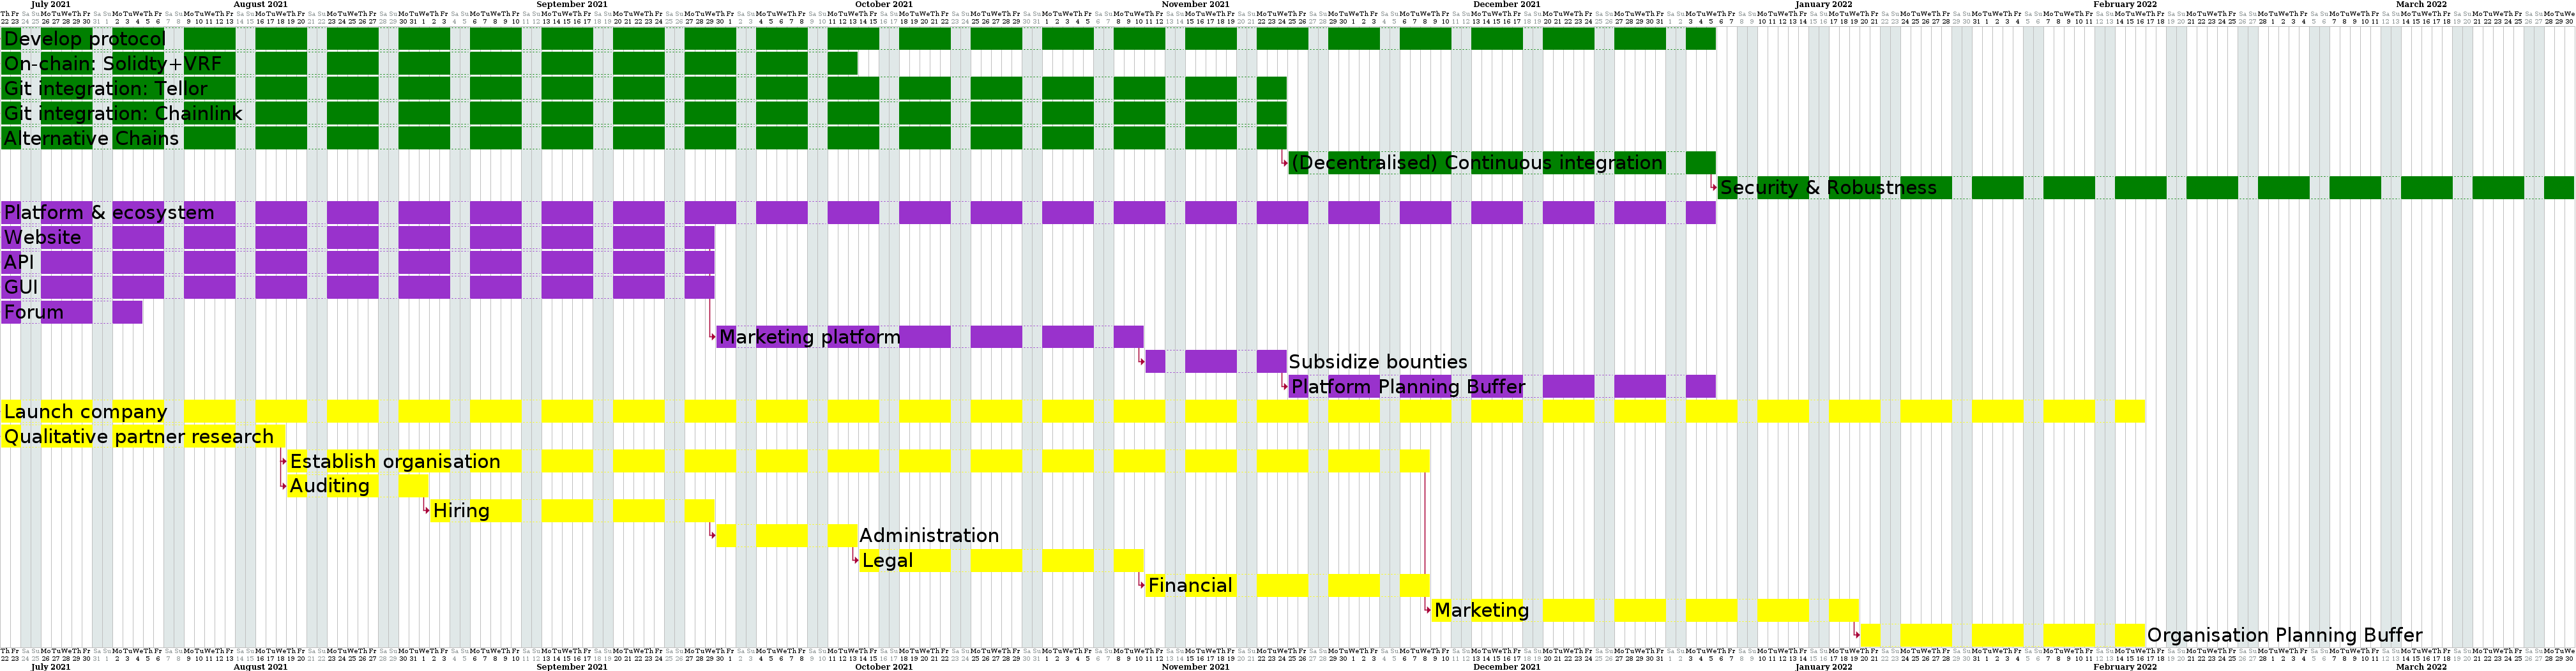
\includepdf{Images/created.png}
\Cref{fig:gantt} contains the Gantt chart that is generated to plan the development of the TruCol company. One can observe that several of the development-activities can be performed in parallel, these are accordingly stacked vertically. Dependencies of outputs of activities imply a "stairway" pattern in the Gantt chart.
\clearpage
\begin{sidewaysfigure}[ht!]
%\begin{sidewaysfigure}[H]
\hspace*{-0cm}
	\ifx\homepath\overleafhome
		%\onecolumn\includegraphics[width=1.0\textwidth]{Images/Diagrams/interaction.png}
		\includegraphics[width=775pt]{Images/Diagrams/gantt.png}
	\else
		\includegraphics[width=775pt]{latex/Images/Diagrams/gantt.png}
		%\onecolumn\includegraphics[width=1.0\textwidth]{latex/Images/Diagrams/interaction.png}
	\fi
    \caption{Gantt chart that is generated to plan the development of the TruCol company. (Source code in appendices, and on github.com/trucol/Roadmap).}
    \label{fig:gantt}
\end{sidewaysfigure}
\clearpage
The description of the activities can be given as:
\subsection{Decentralised Technology Development}
\begin{itemize}
	\item \textbf{Develop protocol} - The programming work and documentation work that is required to render the TruCol protocol to a mature and robust state.
	\item \textbf{On-chain: Solidity+VRF} - Finalisation of the Solidity to Solidity implementation of the TruCol protocol implementation that leverages Chainlinks Verifable Random function (VRF).
	\item \textbf{Git integration: Tellor} - Providing a lower-cost option to the users whilst allowing the user to apply the TruCol protocol in practically any programming language using Tellor oracles that query Git repository content and (build) status.
	\item \textbf{Git integration: Chainlink} - Same as the Tellor option, except using Chainlinks oracles.
	\item \textbf{Alternative Chains} - Implementing the TruCol protocol in alternative chains to facilitate easy use for the users whilst possibly lowering costs and/or modulating the desired levels of decentralisation
	\item \textbf{(Decentralised) Continuous Integration} - Realizing a mature implementation in which the oracles can verify the build status (whether the tests in the smart contract actually passed or not) in a robust fashion. Ideally implementing support for decentralised CIs.
	\item \textbf{Security \& Robustness} - A security audit of the TruCol protocol implementations.
\end{itemize}
\subsection{Platform Development}
\begin{itemize}
	\item \textbf{Platform \& Ecosystem} - Development of the online platform that provides a convenient place for users to use-, discuss- and learn about the TruCol protocol and its various implementations.
	\item \textbf{Website} - Completion of the company website.
	\item \textbf{API} - Application programming interface that allows users to submit contracts using the command line interface (CLI).
	\item \textbf{GUI} - Graphical user interface, that makes it easy and intuitive for new users to start using the TruCol protocol for their applications.
	\item \textbf{Forum} - Environment a-la stack-overflow that cultivates a knowledge base around the use of the TruCol protocol.
	\item \textbf{Marketing platform} - Development of the approach to realise wide-spread adoption of the TruCol eco-system.
	\item \textbf{Subsidize bounties} - Subsidisation of bounties to attract new users to the platform.
	\item \textbf{Platform Planning Buffer} -  A buffer accounting for unknown unknowns/unexpected delays.
\end{itemize}

\subsection{Business Development}
% TODO: make sub-indentation
\begin{itemize}
	\item \textbf{Launch company} -  The administrative and non-technical aspects of growing the TruCol company.
	\item \textbf{Qualitative partner research} - An analysis to identify relevant partners in the growth of our company.
	\item \textbf{Establish Organisation} - organisational aspects of growing the company, with "Auditing, Hiring, Administration, Legal \& Financial tasks as its respective subset".
	\item \textbf{Marketing} - Development of the approach to realise wide-spread adoption of the TruCol protocol whilst realising a steady stream of new customers.
	\item \textbf{Organisation Planning Buffer} -  A buffer accounting for unknown unknowns/unexpected delays.
\end{itemize}

\section{Cost estimates}
After multiplying the amount of labour hours with their respective hourly labour costs, a total estimated labour costs of \euro$470.400,-$ is generated. This is composed of:
\begin{itemize}
	\item Decentralised Tech Development: \euro$252.000,-$
	\item Platform Development: \euro$112.000,-$
	\item Business Development \euro$106.400,-$
\end{itemize}
An additional \euro$100.000,-$ are included for bounty subsidisation and as a buffer, yielding a total expected cost to create a healthy company of roughly \euro$470.000+$\euro$100.000=$\euro$570.000,-$ which is rounded to approximately .6 Meuro.
 %\newpage
  	\section{Sensitivity Analysis \& Monte Carlo Simulation}\label{sec:sensitivity_analysis}
Omitted due to time constraints.
 %\newpage
  	\section{Discussion}\label{sec:discussion}
The hourly wage estimates for the senior decentralised technology development, platform development and business estimates could be refined by using databases of competitive salaries for the respective tasks/work. Furthermore, a refinement of the duration estimates is proposed at the moment the tasks are started, as we expect more relevant information will be available at those times. In addition, external resources should be addressed to check whether any (critical) components are ommited in this Gantt planning.
 %\newpage
  	\section{Conclusion}\label{sec:conclusion}
This document presents the planning to develop the healthy TruCol company within the timeframe of roughly 9 months, and documents the assumptions and methods used to generate this planning. The main tasks in this planning are composed of decentralised technology development, TruCol platform development and business development. A total labour cost of roughly \euro$\labourcosts$ is estimated, and another \euro$\nonlabourcosts$ is estimated for bounty subsidisation and as a buffer.

At the end of this planning, the TruCol company is expected to sustainably operate, generating ROI. Our aim is to gradually increase the cultivation of the diversification potential of the TruCol protocol at this point, whilst starting to develop a strategy to develop our own in-house automation/AI-engine based on the dataset that we continuously grow.
 %\newpage
\else
    % Local compilation
    \input{latex/Chapters/0_introduction.tex} %\newpage
  	\section{Assumptions}\label{sec:assumptions}
\subsection{Decentralisation Developer Wages}
The hourly wage of the developers working on decentralised technology is based on a mixture of ± 3 junior developers working at \euro 100.000,- per year, and 2 senior developers working at \euro 200.000,- per year. This yields an average developer cost of 
\begin{equation}
	\frac{3\cdot 50+2\cdot 100}{5}=\frac{350}{5}=\textup{\euro}70,-
\end{equation}
The datapoints used to come to this estimate are the promoted starting wages for Junior Developers/Engineers at Optiver in Amsterdam, Think-cell in Berlin, and a third Zurich company, which all ranged between 80 to 120k at the time of inspection (Around March 2021). No proper datapoint is used to estimate the salary of the senior developers. Previous experience in co-working with senior developers led to an estimate that their hourly contributions are at least twice as valuable as that of a junior developer. Another indicator for the doubling in wage between junior and senior dev may be the hear-say high demand in solidity/decentralisation developers.

The 70,- hourly wage is interpreted as \euro$75,-$ per hour to be on the conservative side of estimates.
\subsection{Website/Platform Wages}
The website+API+GUI development is estimated at \euro$40$ per hour. This estimate is based on a reduced hourly wage of the junior decentralised technology developers (from \euro$50,-$ to \euro$40,-$). Some of the development costs for these activities may be performed at a lower hourly cost price, this platform development work also contains UX design. And excellent UX design is quite costly, hence the average hourly wage for this estimate is kept at \euro$40,-$.

\subsection{Business wages}
The hourly wages for the business development side of our company is estimated at \euro$35,-$ per hour. This estimate is based on a reduced hourly wage of the junior platform developers (from \euro$40,-$ to \euro$35,-$).

\subsection{Activity durations}
The estimates for the durations of the activities for both decentralised technology development as well as ecosystem development are extrapolations of our experience in developing in these disciplines. The business development activities durations are based roughly on estimating what those activities entail and how long it would take to complete them. %\newpage
  	\section{Cost Model Description}\label{sec:model_description}
The total costs are computed based on two factors.
\begin{itemize}
	\item The cumulative amount of human labour hours that are planned to be executed, multiplied with their respective hourly wage costs as specified in \cref{sec:assumptions}.
	\item A combination of bounty subsidisation and buffer costs of \euro$100.000,-$ are estimated to generate wide-spread adoption of the TruCol protocol.
\end{itemize}
 %\newpage
  	\section{Results}\label{sec:results}
%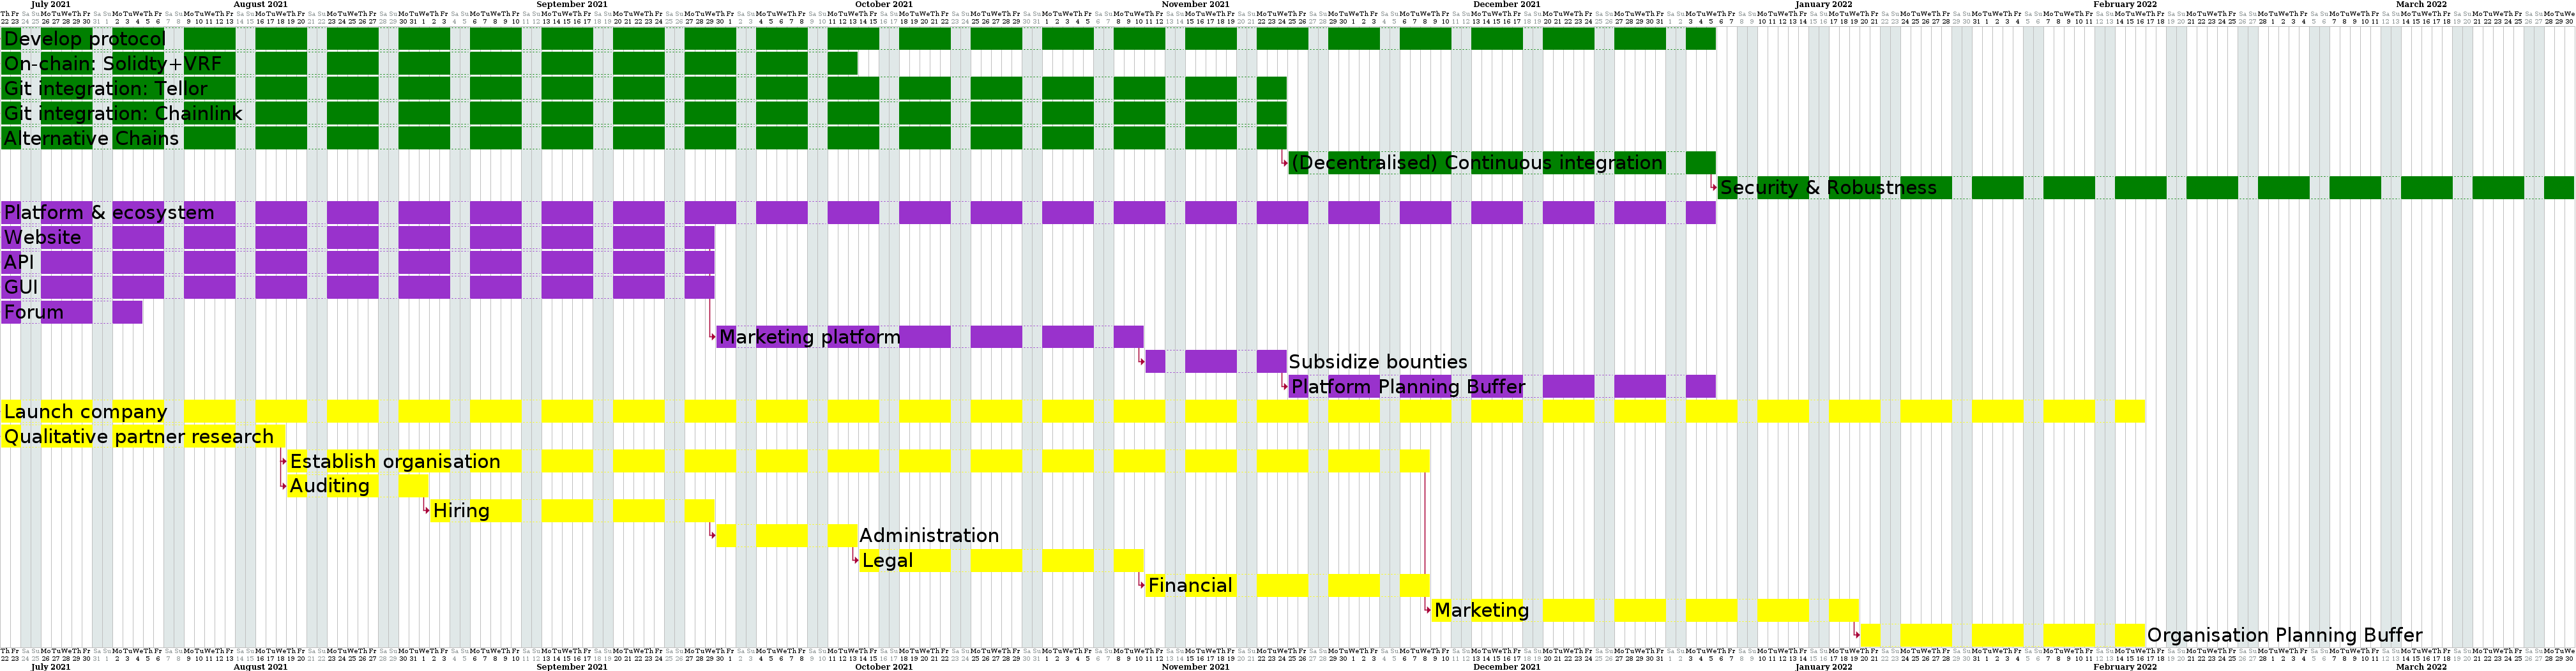
\includepdf{Images/created.png}
\Cref{fig:gantt} contains the Gantt chart that is generated to plan the development of the TruCol company. One can observe that several of the development-activities can be performed in parallel, these are accordingly stacked vertically. Dependencies of outputs of activities imply a "stairway" pattern in the Gantt chart.
\clearpage
\begin{sidewaysfigure}[ht!]
%\begin{sidewaysfigure}[H]
\hspace*{-0cm}
	\ifx\homepath\overleafhome
		%\onecolumn\includegraphics[width=1.0\textwidth]{Images/Diagrams/interaction.png}
		\includegraphics[width=775pt]{Images/Diagrams/gantt.png}
	\else
		\includegraphics[width=775pt]{latex/Images/Diagrams/gantt.png}
		%\onecolumn\includegraphics[width=1.0\textwidth]{latex/Images/Diagrams/interaction.png}
	\fi
    \caption{Gantt chart that is generated to plan the development of the TruCol company. (Source code in appendices, and on github.com/trucol/Roadmap).}
    \label{fig:gantt}
\end{sidewaysfigure}
\clearpage
The description of the activities can be given as:
\subsection{Decentralised Technology Development}
\begin{itemize}
	\item \textbf{Develop protocol} - The programming work and documentation work that is required to render the TruCol protocol to a mature and robust state.
	\item \textbf{On-chain: Solidity+VRF} - Finalisation of the Solidity to Solidity implementation of the TruCol protocol implementation that leverages Chainlinks Verifable Random function (VRF).
	\item \textbf{Git integration: Tellor} - Providing a lower-cost option to the users whilst allowing the user to apply the TruCol protocol in practically any programming language using Tellor oracles that query Git repository content and (build) status.
	\item \textbf{Git integration: Chainlink} - Same as the Tellor option, except using Chainlinks oracles.
	\item \textbf{Alternative Chains} - Implementing the TruCol protocol in alternative chains to facilitate easy use for the users whilst possibly lowering costs and/or modulating the desired levels of decentralisation
	\item \textbf{(Decentralised) Continuous Integration} - Realizing a mature implementation in which the oracles can verify the build status (whether the tests in the smart contract actually passed or not) in a robust fashion. Ideally implementing support for decentralised CIs.
	\item \textbf{Security \& Robustness} - A security audit of the TruCol protocol implementations.
\end{itemize}
\subsection{Platform Development}
\begin{itemize}
	\item \textbf{Platform \& Ecosystem} - Development of the online platform that provides a convenient place for users to use-, discuss- and learn about the TruCol protocol and its various implementations.
	\item \textbf{Website} - Completion of the company website.
	\item \textbf{API} - Application programming interface that allows users to submit contracts using the command line interface (CLI).
	\item \textbf{GUI} - Graphical user interface, that makes it easy and intuitive for new users to start using the TruCol protocol for their applications.
	\item \textbf{Forum} - Environment a-la stack-overflow that cultivates a knowledge base around the use of the TruCol protocol.
	\item \textbf{Marketing platform} - Development of the approach to realise wide-spread adoption of the TruCol eco-system.
	\item \textbf{Subsidize bounties} - Subsidisation of bounties to attract new users to the platform.
	\item \textbf{Platform Planning Buffer} -  A buffer accounting for unknown unknowns/unexpected delays.
\end{itemize}

\subsection{Business Development}
% TODO: make sub-indentation
\begin{itemize}
	\item \textbf{Launch company} -  The administrative and non-technical aspects of growing the TruCol company.
	\item \textbf{Qualitative partner research} - An analysis to identify relevant partners in the growth of our company.
	\item \textbf{Establish Organisation} - organisational aspects of growing the company, with "Auditing, Hiring, Administration, Legal \& Financial tasks as its respective subset".
	\item \textbf{Marketing} - Development of the approach to realise wide-spread adoption of the TruCol protocol whilst realising a steady stream of new customers.
	\item \textbf{Organisation Planning Buffer} -  A buffer accounting for unknown unknowns/unexpected delays.
\end{itemize}

\section{Cost estimates}
After multiplying the amount of labour hours with their respective hourly labour costs, a total estimated labour costs of \euro$470.400,-$ is generated. This is composed of:
\begin{itemize}
	\item Decentralised Tech Development: \euro$252.000,-$
	\item Platform Development: \euro$112.000,-$
	\item Business Development \euro$106.400,-$
\end{itemize}
An additional \euro$100.000,-$ are included for bounty subsidisation and as a buffer, yielding a total expected cost to create a healthy company of roughly \euro$470.000+$\euro$100.000=$\euro$570.000,-$ which is rounded to approximately .6 Meuro.
 %\newpage
  	\section{Sensitivity Analysis \& Monte Carlo Simulation}\label{sec:sensitivity_analysis}
Omitted due to time constraints.
 %\newpage
  	\section{Discussion}\label{sec:discussion}
The hourly wage estimates for the senior decentralised technology development, platform development and business estimates could be refined by using databases of competitive salaries for the respective tasks/work. Furthermore, a refinement of the duration estimates is proposed at the moment the tasks are started, as we expect more relevant information will be available at those times. In addition, external resources should be addressed to check whether any (critical) components are ommited in this Gantt planning.
 %\newpage
  	\section{Conclusion}\label{sec:conclusion}
This document presents the planning to develop the healthy TruCol company within the timeframe of roughly 9 months, and documents the assumptions and methods used to generate this planning. The main tasks in this planning are composed of decentralised technology development, TruCol platform development and business development. A total labour cost of roughly \euro$\labourcosts$ is estimated, and another \euro$\nonlabourcosts$ is estimated for bounty subsidisation and as a buffer.

At the end of this planning, the TruCol company is expected to sustainably operate, generating ROI. Our aim is to gradually increase the cultivation of the diversification potential of the TruCol protocol at this point, whilst starting to develop a strategy to develop our own in-house automation/AI-engine based on the dataset that we continuously grow.
 %\newpage
\fi

% Include bibliography
\bibliographystyle{plain} %plain style
\bibliography{references}
\addcontentsline{toc}{chapter}{Bibliography}

%\begin{appendices}
%  \ifx\homepath\overleafhome
%      % Overleaf compilation.
%      \section{Appendix \_\_main\_\_.py}\label{app:a}
\IfFileExists{latex/project1/../../code/project1/src/__main__.py}{
\pythonexternal{latex/project1/../../code/project1/src/__main__.py}
}{
\pythonexternal{../../code/project1/src/__main__.py}
}
 %\newpage
%      \section{Appendix Main.py}\label{app:b}
\IfFileExists{latex/project1/../../code/project1/src/Main.py}{
\pythonexternal{latex/project1/../../code/project1/src/Main.py}
}{
\pythonexternal{../../code/project1/src/Main.py}
}
 %\newpage
%  \else
%      % Local compilation
%      \section{Appendix \_\_main\_\_.py}\label{app:a}
%\IfFileExists{latex/project1/../../code/project1/src/__main__.py}{
%\pythonexternal{latex/project1/../../code/project1/src/__main__.py}
%}{
%\pythonexternal{../../code/project1/src/__main__.py}
%}
 %\newpage
%      \section{Appendix Main.py}\label{app:b}
%\IfFileExists{latex/project1/../../code/project1/src/Main.py}{
%\pythonexternal{latex/project1/../../code/project1/src/Main.py}
%}{
%\pythonexternal{../../code/project1/src/Main.py}
%}
 %\newpage
%  \fi
%\end{appendices}
\end{document}
